% ============================================================
% Manuscript prepared for Annals of Telecommunications
% Springer Nature LaTeX template, iicol option
%
% IMPORTANT:
% 1. Download sn-jnl.cls from the official Springer template.
% 2. Replace every visible TODO before submission.
% 3. Verify all references, affiliations, funding statements,
%    author contributions, data, and numerical results.
% ============================================================

\documentclass[pdflatex,sn-mathphys-num,iicol,oneside]{sn-jnl}

% \jyear{2026}

\usepackage{amsmath}
\usepackage{amssymb}
\usepackage{bm}
\usepackage{booktabs}
\usepackage{multirow}
\usepackage{array}
\usepackage{xcolor}
\usepackage{tikz}
\usepackage{url}

\usetikzlibrary{arrows.meta,positioning,fit,shapes.geometric}

% Visible placeholders: remove before submission.
\newcommand{\TODO}[1]{\textcolor{red}{\textbf{[TODO: #1]}}}
\newcommand{\method}{\textsc{VeriXApp}}
\newcommand{\mirage}{\textsc{Mirage-R}}

\newtheorem{proposition}{Proposition}
\newtheorem{definition}{Definition}
\newtheorem{remark}{Remark}

\raggedbottom

\begin{document}

\title[Finite-Domain Conflict-Free xApp Coordination]{\vspace*{-20pt}Finite-Domain Conflict-Free xApp Coordination: A Hybrid Continuous-Inference and Exact-Repair Framework for O-RAN}

% ============================================================
% Authors
% ============================================================

\author*[1]{\fnm{Lillia} \sur{Ouali}}\email{lillia.ouali@univ-bejaia.dz}
\author[2]{\fnm{Madani} \sur{Bezoui}}\email{mbezoui@cesi.fr}
\author[1]{\fnm{Kamal} \sur{Amroun}}\email{kamal.amroun@univ-bejaia.dz}
\author[3]{\fnm{Ahcene} \sur{Bounceur}}\email{abounceur@sharjah.ac.ae}

\affil*[1]{\orgdiv{Department of Computer Science}, \orgname{University of Bejaia}, \orgaddress{\city{Bejaia}, \country{Algeria}}}
\affil[2]{\orgdiv{LINEACT}, \orgname{CESI}, \orgaddress{\city{Nancy}, \country{France}}}
\affil[3]{\orgname{University of Sharjah}, \orgaddress{\city{Sharjah}, \country{United Arab Emirates}}}
\vspace*{-20pt}

% ============================================================
% Abstract: currently approximately 220 words
% ============================================================

\abstract{
The programmability of the Open Radio Access Network (O-RAN)
allows independently developed extended applications, called xApps,
to control radio access network parameters through the near-real-time
RAN Intelligent Controller. However, concurrently deployed xApps may
issue incompatible actions, compete for shared resources, or
indirectly degrade each other's key performance indicators. Existing
conflict-management approaches primarily rely on static priorities,
learned performance predictors, digital twins, or joint training.
This paper investigates a complementary failure mode that arises when
discrete xApp coordination is addressed through continuous
relaxation. We formulate conflict-free xApp arbitration as a
finite-domain constraint optimization problem and characterize
non-integral fixed points of a relation-conditioned
product-of-experts update. Such fractional fixed points represent
stable continuous configurations whose deterministic decoding still
produces an invalid or service-level-agreement-violating control
decision. We then introduce \method, a verified hybrid framework that
combines continuous marginal inference, explicit fixed-point
diagnostics, exact repair of a conflict-induced subproblem, and an
independent decision verifier. The framework distinguishes direct,
indirect, and implicit conflicts and returns a control action only
after validating all registered hard constraints. The experimental
protocol evaluates the approach on reproducible O-RAN scenarios
involving energy saving, mobility robustness, load balancing, power
control, and radio-resource allocation. Comparisons include
uncoordinated execution, static-priority arbitration, continuous-only
coordination, and complete constraint programming.
The results show that continuous-only coordination stalls on
approximately one quarter of decision epochs and reaches only 74.7\%
verified feasibility, whereas \method\ detects and exactly repairs every
stall to attain 100\% verified feasibility, matching complete constraint
programming. On these instances the exact CP-SAT solver is itself fast and
complete, so the continuous stage of \method\ adds latency (median 42~ms)
rather than reducing it; its contribution is the explicit fractional-stall
diagnosis and the independent verification guarantee, with exact repair
confined to a median core of two variables.
}

\keywords{
O-RAN,
xApp conflict management,
near-real-time RIC,
constraint programming,
continuous relaxation,
fractional fixed points
}

\let\origclearpage\clearpage
\let\orignewpage\newpage
\def\clearpage{}
\def\newpage{}
\maketitle
\let\clearpage\origclearpage
\let\newpage\orignewpage

% ============================================================
\section{Introduction}
% ============================================================

Open Radio Access Network (O-RAN) introduces disaggregation,
open interfaces, and programmable control into radio access
networks. A central component of this architecture is the RAN
Intelligent Controller (RIC), which supports applications operating
at different time scales. The non-real-time RIC hosts rApps, whereas
the near-real-time RIC hosts extended applications, referred to as
xApps \cite{polese2023oran}.

An xApp can implement a control function such as traffic steering,
mobility optimization, interference coordination, energy saving, or
radio-resource allocation. The E2 interface allows these applications
to receive network measurements and issue control requests to E2
nodes. This flexibility enables a multi-vendor ecosystem but also
creates a fundamental coordination problem: independently developed
xApps may simultaneously attempt to control the same network
parameter or pursue mutually incompatible performance objectives.

The O-RAN Alliance identifies conflict mitigation between xApps as a
specific function of the near-real-time RIC
\cite{oran2024conflict}. Existing studies distinguish direct,
indirect, and implicit conflicts
\cite{adamczyk2023conflict,wadud2024qacm}.
Direct conflicts occur when xApps request incompatible values for the
same network control parameter. Indirect conflicts arise when
different parameters controlled by different xApps affect a common
key performance measurement. Implicit conflicts are more difficult
to observe because different parameters and performance indicators
interact through the network dynamics.

Several approaches have been developed for conflict detection,
profiling, and resolution. These include static priorities,
QoS-aware optimization, digital-twin-based evaluation, application
profiling, game-theoretic mechanisms, and reinforcement learning
\cite{wadud2024qacm,prever2025pacifista,
giannopoulos2025comix,wadud2025mobility}.
These methods provide important conflict-management mechanisms.
However, comparatively little attention has been given to the
behaviour of continuous relaxations when the final RAN control
decision must belong to a finite set.

This paper considers xApp coordination as a finite-domain constraint
optimization problem. Each decision variable represents an accepted
xApp action, an execution slot, a target cell, a power level, or a
resource-allocation configuration. A continuous relaxation assigns a
probability distribution to every variable and iteratively combines
the local recommendations of conflict constraints.

The central observation is that such an iteration may stop at a
non-integral configuration. The continuous state no longer changes,
but deterministic decoding produces an invalid or SLA-violating
decision. We call this configuration a \emph{fractional fixed point}.
The concept concerns the fixed points of the implemented update map;
it is not presented as a stationary point of an unspecified global
optimization objective.

To address this failure mode, we introduce \method, a hybrid
coordination framework composed of four stages:

\begin{enumerate}
    \item finite-domain modelling of candidate xApp actions;
    \item continuous relation-conditioned marginal inference;
    \item explicit fractional-fixed-point detection;
    \item exact local repair followed by independent verification.
\end{enumerate}

The main contributions are as follows.

\begin{itemize}
    \item We formulate conflict-free multi-xApp coordination as a
    finite-domain constraint optimization problem that supports
    direct, indirect, and implicit conflict relations.

    \item We characterize a class of fractional fixed points in the
    continuous coordination map and show how they can yield an
    infeasible decoded action.

    \item We propose an exact local-repair mechanism that extracts a
    conflict-induced subproblem instead of adding uncorrected
    overlapping factors to the continuous model.

    \item We define a verified decision pipeline: no coordinated
    action is forwarded to the RAN unless an independent verifier
    confirms all registered hard constraints.

    \item We specify a reproducible evaluation protocol covering
    feasibility, SLA satisfaction, network utility, control latency,
    stability, and computational overhead.
\end{itemize}

The remainder of this paper is organized as follows.
Section~\ref{sec:background} reviews O-RAN conflict management.
Section~\ref{sec:model} presents the system and conflict models.
Section~\ref{sec:method} introduces \method.
Section~\ref{sec:analysis} analyzes fractional fixed points. Section~\ref{sec:experiments} defines the experimental protocol. Section~\ref{sec:results} presents the results.
Section~\ref{sec:limitations} discusses limitations, and
Section~\ref{sec:conclusion} concludes the paper.

% ============================================================
\section{Background and Related Work}
\label{sec:background}
% ============================================================

\subsection{O-RAN control architecture}

The O-RAN architecture includes the Service Management and
Orchestration framework, the non-real-time RIC, the near-real-time
RIC, and disaggregated RAN components such as the O-CU, O-DU, and
O-RU \cite{polese2023oran}.

The near-real-time RIC supports control loops typically operating
between tens of milliseconds and one second. xApps subscribe to
measurements, process network context, and issue E2 control requests.
Open experimental frameworks such as ColO-RAN, OpenRAN Gym, and
FlexRIC facilitate the development and evaluation of programmable
RAN controllers
\cite{polese2022coloran,bonati2023openrangym,
schmidt2021flexric}. Recent work has also compared simulated,
emulated, hybrid, and hardware-based O-RAN experimentation platforms
under resource constraints \cite{navarro2026testbeds}.

Figure~\ref{fig:architecture} shows the position of the proposed
conflict-management component. The component intercepts candidate
control requests before they are forwarded through the E2 interface.

\begin{figure*}[t]
\centering
\resizebox{\textwidth}{!}{%
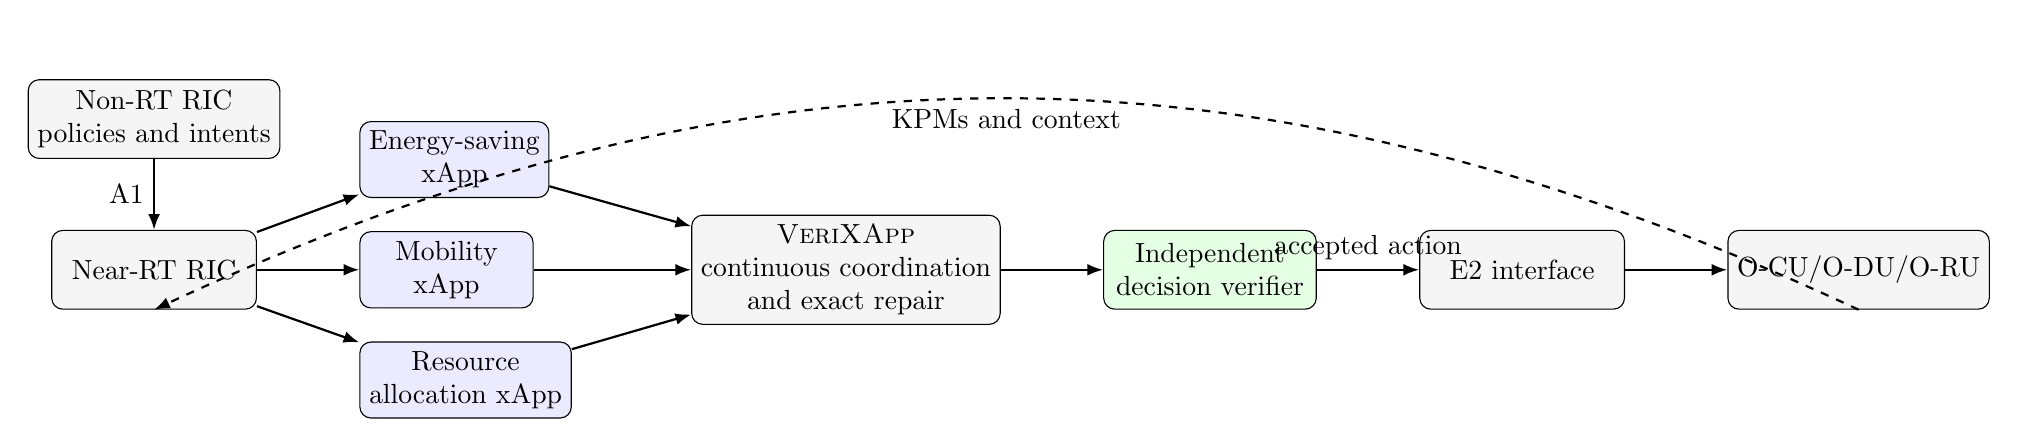
\begin{tikzpicture}[
    node distance=9mm and 13mm,
    block/.style={
        draw,
        rounded corners,
        align=center,
        minimum width=26mm,
        minimum height=10mm,
        fill=gray!8
    },
    app/.style={
        draw,
        rounded corners,
        align=center,
        minimum width=22mm,
        minimum height=9mm,
        fill=blue!8
    },
    verify/.style={
        draw,
        rounded corners,
        align=center,
        minimum width=27mm,
        minimum height=10mm,
        fill=green!10
    },
    arrow/.style={-{Latex[length=2mm]},thick}
]

\node[block] (nonrt) {Non-RT RIC\\policies and intents};
\node[block, below=of nonrt] (near) {Near-RT RIC};

\node[app, right=of near, yshift=14mm] (x1) {Energy-saving\\xApp};
\node[app, right=of near] (x2) {Mobility\\xApp};
\node[app, right=of near, yshift=-14mm] (x3) {Resource\\allocation xApp};

\node[block, right=20mm of x2] (cm) {
\method\\
continuous coordination\\
and exact repair
};

\node[verify, right=of cm] (verifier) {
Independent\\
decision verifier
};

\node[block, right=of verifier] (e2) {E2 interface};
\node[block, right=of e2] (ran) {O-CU/O-DU/O-RU};

\draw[arrow] (nonrt) -- node[left]{A1} (near);
\draw[arrow] (near) -- (x1);
\draw[arrow] (near) -- (x2);
\draw[arrow] (near) -- (x3);

\draw[arrow] (x1) -- (cm);
\draw[arrow] (x2) -- (cm);
\draw[arrow] (x3) -- (cm);

\draw[arrow] (cm) -- (verifier);
\draw[arrow] (verifier) -- node[above]{accepted action} (e2);
\draw[arrow] (e2) -- (ran);

\draw[arrow,dashed] (ran.south) to[bend right=25]
node[below]{KPMs and context} (near.south);

\end{tikzpicture}
}
\caption{
Position of \method\ in the near-real-time RIC control path.
Candidate xApp actions are coordinated and independently verified
before being forwarded to an E2 node.
}
\label{fig:architecture}
\end{figure*}

\subsection{xApp conflict types}

Let $\mathcal{A}=\{1,\ldots,n\}$ denote the set of active xApps,
$\mathcal{P}$ the set of network control parameters, and
$\mathcal{K}$ the set of monitored key performance measurements.

A direct conflict occurs when two or more xApps propose incompatible
values for the same parameter. For example, a coverage xApp may
request a transmission-power increase while an interference or
energy-saving xApp requests a decrease.

An indirect conflict occurs when xApps modify different parameters
that influence the same KPM. For example, a load-balancing xApp may
modify cell individual offsets while a mobility xApp modifies
handover thresholds. Both actions affect cell association and load.

An implicit conflict occurs when actions targeting distinct
parameters and KPMs interact through the RAN dynamics. For example,
putting a cell into a low-energy state may reduce energy consumption
but increase mobility failures or violate slice throughput
requirements.

The three categories are not equally observable. Direct conflicts can
often be verified syntactically from the proposed parameter values.
Indirect conflicts require a registered parameter--KPM dependency
model. Implicit conflicts require either a validated impact model, a
digital twin, an emulator, or conservative operator rules.

\subsection{Conflict-management approaches}

Adamczyk and Kliks proposed a conflict-mitigation framework embedded
in the near-real-time RIC, including conflict detection and
resolution mechanisms \cite{adamczyk2023conflict}. QACM formulates
resolution as a QoS-aware optimization problem that seeks to satisfy
the requirements of as many xApps as possible
\cite{wadud2024qacm}.

PACIFISTA profiles O-RAN applications in a controlled environment and
uses statistical models and hierarchical graphs to characterize
conflicts before deployment \cite{prever2025pacifista}. COMIX
combines a conflict-management framework with a network digital twin
for multi-channel power control
\cite{giannopoulos2025comix}. Mobility-driven energy-saving
experiments have also been used to study direct, indirect, and
implicit conflicts \cite{wadud2025mobility}.

The present work is complementary. It does not attempt to replace
profiling, prediction, or digital twins. Instead, it addresses what
happens after candidate actions and conflict relations have been
registered: a continuous coordinator may converge to a non-integral
state that cannot be decoded safely.

% ============================================================
\section{System and Conflict Model}
\label{sec:model}
% ============================================================

\subsection{Decision epochs and candidate actions}

The near-real-time RIC operates over decision epochs
$t=1,\ldots,T$. At epoch $t$, each active xApp $i$ produces a finite
set of candidate actions

\begin{equation}
D_i^t =
\left\{
a_{i,1}^t,\ldots,a_{i,d_i}^t
\right\}.
\end{equation}

An action may represent:

\begin{itemize}
    \item accepting or rejecting a control request;
    \item selecting a target cell;
    \item assigning an execution slot;
    \item selecting a discrete transmission-power level;
    \item applying a configured handover offset;
    \item selecting a radio-resource-allocation profile;
    \item executing a safe no-operation action.
\end{itemize}

The discrete decision variable $x_i^t\in D_i^t$ represents the
coordinated action selected for xApp $i$. The time index is omitted
when a single decision epoch is considered.

\subsection{Conflict relations}

A constraint $c\in\mathcal{C}$ has scope
$S_c\subseteq\mathcal{A}$ and an allowed relation

\begin{equation}
R_c(\bm{s}_t)
\subseteq
\prod_{i\in S_c}D_i,
\end{equation}

where $\bm{s}_t$ denotes the observed network context.

An assignment $\bm{x}$ satisfies constraint $c$ if

\begin{equation}
\bm{x}_{S_c}\in R_c(\bm{s}_t).
\end{equation}

Relations may be binary or higher-order. Context-dependent relations
can be generated from:

\begin{enumerate}
    \item operator policies;
    \item parameter-ownership declarations;
    \item SLA and QoS thresholds;
    \item validated xApp profiles;
    \item a calibrated network simulator or digital twin;
    \item conservative safety rules.
\end{enumerate}

We distinguish hard and soft constraints. A hard constraint must be
satisfied before an action is forwarded to the RAN. A soft constraint
contributes to the utility but may be violated at a specified cost.

\subsection{Utility and SLA satisfaction}

Let $u_i(a_i,\bm{s}_t)$ denote the predicted or measured utility of
selecting action $a_i$ for xApp $i$. Let
$\omega_i\geq 0$ denote the operator-defined priority.

The aggregate utility is

\begin{equation}
U(\bm{x},\bm{s}_t)
=
\sum_{i\in\mathcal{A}}
\omega_i u_i(x_i,\bm{s}_t)
-
\sum_{q\in\mathcal{Q}}
\lambda_q
v_q(\bm{x},\bm{s}_t),
\label{eq:utility}
\end{equation}

where $v_q$ is a non-negative soft-violation penalty and
$\lambda_q$ is its weight.

The optimization problem is

\begin{align}
\max_{\bm{x}}\quad&
U(\bm{x},\bm{s}_t)
\label{eq:problem-objective}\\
\text{s.t.}\quad&
x_i\in D_i,
&& i\in\mathcal{A},
\label{eq:problem-domain}\\
&
\bm{x}_{S_c}\in R_c(\bm{s}_t),
&& c\in\mathcal{C}_{\mathrm{hard}}.
\label{eq:problem-hard}
\end{align}

Problem~\eqref{eq:problem-objective}--\eqref{eq:problem-hard} is a
finite-domain constraint optimization problem. It may be solved
exactly for small instances, but its combinatorial size grows with
the number of xApps, cells, resources, and candidate actions.

\subsection{Conflict-graph representation}

We define a heterogeneous dependency graph

\begin{equation}
G_t=(V_t,E_t),
\end{equation}

whose nodes include xApps, control parameters, constraints, and KPMs.
An edge records that:

\begin{itemize}
    \item an xApp controls a parameter;
    \item a parameter influences a KPM;
    \item a constraint contains a decision variable;
    \item a KPM belongs to an SLA.
\end{itemize}

The graph is used to identify the variables involved in a detected
conflict and to construct the exact local-repair subproblem.

% ============================================================
\section{The \method\ Coordination Framework}
\label{sec:method}
% ============================================================

\subsection{Continuous lifting}

Each discrete variable $x_i$ is lifted to a categorical marginal

\begin{equation}
\bm{p}_i
\in
\Delta_{d_i}
=
\left\{
\bm{p}\in\mathbb{R}_{+}^{d_i}:
\sum_{a\in D_i}p(a)=1
\right\}.
\end{equation}

The value $p_i(a)$ represents the current continuous preference for
action $a\in D_i$. The joint continuous state is

\begin{equation}
\bm{p}
=
(\bm{p}_1,\ldots,\bm{p}_n)
\in
\prod_{i=1}^{n}\Delta_{d_i}.
\end{equation}

Marginals are initialized from xApp confidence values when available.
Otherwise, they are initialized uniformly and perturbed with small
seeded noise to break exact symmetries.

\subsection{Relation-conditioned messages}

For every hard relation $R_c$ and allowed tuple
$\bm{z}\in R_c$, define

\begin{equation}
w_c(\bm{z};\bm{p})
=
\exp\left[
\frac{1}{\tau}
\left(
\sum_{j\in S_c}
\log\max\{p_j(z_j),\varepsilon\}
+
\gamma_c u_c(\bm{z})
\right)
\right],
\label{eq:tuple-weight}
\end{equation}

where:

\begin{itemize}
    \item $\tau>0$ is a temperature;
    \item $\varepsilon>0$ prevents logarithms of zero;
    \item $u_c$ is an optional local utility;
    \item $\gamma_c$ controls the influence of this utility.
\end{itemize}

The relation-conditioned message from constraint $c$ to variable $i$
is

\begin{equation}
\pi_{c\rightarrow i}(a)
=
\frac{
\displaystyle
\sum_{\substack{\bm{z}\in R_c\\z_i=a}}
w_c(\bm{z};\bm{p})
}{
\displaystyle
\sum_{\bm{z}\in R_c}
w_c(\bm{z};\bm{p})
}.
\label{eq:message}
\end{equation}

If the constraint allows no valid tuples, the model is locally infeasible. Numerical underflow during the marginalization is prevented through log-sum-exp normalization.

\subsection{Geometric consensus}

Let $\mathcal{C}_i$ be the set of constraints incident to variable
$i$. The log-domain consensus is

\begin{equation}
\ell_i(a)
=
\alpha\log\max\{p_i(a),\varepsilon\}
+
\sum_{c\in\mathcal{C}_i}
\eta_{c,i}
\log\max\{\pi_{c\rightarrow i}(a),\varepsilon\},
\label{eq:consensus}
\end{equation}

where $\alpha\geq 0$ is an inertia parameter and

\begin{equation}
\eta_{c,i}>0,
\qquad
\sum_{c\in\mathcal{C}_i}\eta_{c,i}=1.
\end{equation}

The normalized consensus marginal is

\begin{equation}
\widehat{p}_i(a)
=
\frac{\exp(\ell_i(a))}
{\sum_{b\in D_i}\exp(\ell_i(b))}.
\end{equation}

A polarization step is then applied:

\begin{equation}
q_i(a)
=
\frac{\widehat{p}_i(a)^{\beta}}
{\sum_{b\in D_i}\widehat{p}_i(b)^{\beta}},
\qquad \beta\geq 1.
\label{eq:polarization}
\end{equation}

Finally, clipping and renormalization give

\begin{equation}
p_i^{+}(a)
=
\frac{\max\{q_i(a),\varepsilon\}}
{\sum_{b\in D_i}\max\{q_i(b),\varepsilon\}}.
\label{eq:clipping}
\end{equation}

Equations~\eqref{eq:tuple-weight}--\eqref{eq:clipping} define the
continuous update map

\begin{equation}
T:\bm{p}\mapsto\bm{p}^{+}.
\end{equation}

No claim is made that $T$ is an exact ascent or descent step for a
global objective.

\subsection{Decoding}

The discrete candidate is obtained by deterministic decoding:

\begin{equation}
\widehat{x}_i
=
\arg\max_{a\in D_i}p_i(a).
\label{eq:decode}
\end{equation}

Ties are broken using a fixed, documented order. The decoded candidate
is not considered valid until it has passed the independent verifier.

\subsection{Fixed-point diagnostics}

The update residual is

\begin{equation}
\rho(\bm{p})
=
\max_{i\in\mathcal{A}}
\left\|
T_i(\bm{p})-\bm{p}_i
\right\|_1.
\label{eq:residual}
\end{equation}

The fractionality score is

\begin{equation}
\phi(\bm{p})
=
\frac{1}{|\mathcal{A}|}
\sum_{i\in\mathcal{A}}
\left(
1-\max_{a\in D_i}p_i(a)
\right).
\label{eq:fractionality}
\end{equation}

Let

\begin{equation}
V(\widehat{\bm{x}})
=
\sum_{c\in\mathcal{C}_{\mathrm{hard}}}
\mathbf{1}
\left[
\widehat{\bm{x}}_{S_c}
\notin R_c(\bm{s}_t)
\right]
\label{eq:violations}
\end{equation}

be the number of violated hard relations.

\begin{definition}[Operational fractional stall]
A continuous state $\bm{p}$ is classified as an operational
fractional stall if

\begin{equation}
\rho(\bm{p})\leq\delta_{\rho},
\qquad
\phi(\bm{p})\geq\delta_{\phi},
\qquad
V(\widehat{\bm{x}})>0.
\end{equation}
\end{definition}

This operational test does not prove exact equality
$T(\bm{p})=\bm{p}$. It identifies a numerically stable, non-integral,
and operationally invalid state.

\subsection{Conflict-induced exact repair}

When the decoded candidate is invalid, the framework constructs a
repair core. Let

\begin{equation}
\mathcal{C}^{0}
=
\left\{
c\in\mathcal{C}_{\mathrm{hard}}:
\widehat{\bm{x}}_{S_c}\notin R_c
\right\}
\end{equation}

be the set of violated constraints. The initial repair variables are

\begin{equation}
\mathcal{A}^{0}
=
\bigcup_{c\in\mathcal{C}^{0}}S_c.
\end{equation}

The core is optionally expanded by $h$ hops in the conflict graph to
include neighbouring xApps and constraints. Variables outside the
core are fixed to their decoded values. The induced subproblem is
then passed to an exact solver.

The repair objective is lexicographic:

\begin{enumerate}
    \item satisfy every hard relation in the repair core;
    \item minimize the number of changes relative to
    $\widehat{\bm{x}}$;
    \item maximize the utility in
    Equation~\eqref{eq:utility}.
\end{enumerate}

The repair solver is subject to a strict time limit compatible with
the control-loop budget. If repair fails, \method\ selects a
pre-registered safe fallback action, such as rejecting the conflicting
requests or retaining the previous verified configuration.

\subsection{Independent verifier}

The verifier is implemented separately from both the continuous
coordinator and the exact repair adapter. It receives:

\begin{itemize}
    \item the network context identifier;
    \item the selected actions;
    \item the registered domains;
    \item the hard relations;
    \item the applicable SLA thresholds.
\end{itemize}

It evaluates every hard constraint directly. The accepted-decision
set is

\begin{equation}
\mathcal{F}(\bm{s}_t)
=
\left\{
\bm{x}:
x_i\in D_i,
\;
\bm{x}_{S_c}\in R_c(\bm{s}_t),
\;
\forall c\in\mathcal{C}_{\mathrm{hard}}
\right\}.
\end{equation}

\begin{proposition}[Decision soundness]
If \method\ forwards an action $\bm{x}$ to the E2 interface, then
$\bm{x}\in\mathcal{F}(\bm{s}_t)$ relative to the registered domains,
relations, context, and verifier semantics.
\end{proposition}

\begin{proof}
By construction, the framework forwards a candidate only if the
independent verifier accepts it. The verifier accepts a candidate
only after checking domain membership and every registered hard
relation. Therefore, an action forwarded by the framework belongs to
$\mathcal{F}(\bm{s}_t)$.
\end{proof}

This proposition does not prove that the registered model perfectly
represents the physical RAN. Model validity and decision verification
are separate properties.

% ============================================================
\section{Fractional-Fixed-Point Analysis}
\label{sec:analysis}
% ============================================================

\subsection{Illustrative xApp arbitration motif}

Consider two xApp control requests that must be assigned to two
different execution slots. For example, the requests may modify a
shared parameter and must be temporally separated to prevent a direct
conflict.

Let

\begin{equation}
D_1=D_2=\{0,1\}
\end{equation}

and define the allowed relation

\begin{equation}
R_{\neq}
=
\{(0,1),(1,0)\}.
\end{equation}

Write the two marginals as

\begin{equation}
\bm{p}_1=(s,1-s),
\qquad
\bm{p}_2=(t,1-t).
\end{equation}

At $\tau=1$, $\beta=1$, $\alpha=0$, and without clipping, the update is

\begin{align}
s^{+}
&=
\frac{s(1-t)}
{s(1-t)+(1-s)t},
\label{eq:s-update}
\\
t^{+}
&=
\frac{t(1-s)}
{t(1-s)+(1-t)s}.
\label{eq:t-update}
\end{align}

\begin{proposition}[Fractional xApp arbitration point]
The interior fixed point of
Equations~\eqref{eq:s-update}--\eqref{eq:t-update} is

\begin{equation}
(s,t)=\left(\frac{1}{2},\frac{1}{2}\right).
\end{equation}

The Jacobian at this point is

\begin{equation}
J=
\begin{bmatrix}
1 & -1\\
-1 & 1
\end{bmatrix},
\end{equation}

whose eigenvalues are $0$ and $2$. Therefore, the uniform
configuration is a fractional saddle. Under deterministic identical
tie-breaking, both variables decode to the same slot and violate
$R_{\neq}$.
\end{proposition}

\begin{proof}
At an interior fixed point,
Equation~\eqref{eq:s-update} requires

\begin{equation}
s(1-t)+(1-s)t=1-t.
\end{equation}

Symmetrically,

\begin{equation}
t(1-s)+(1-t)s=1-s.
\end{equation}

Subtracting the two equations gives $s=t$. Substitution yields

\begin{equation}
2s^2-3s+1=0.
\end{equation}

Its interior solution is $s=1/2$. Differentiating the update map at
$(1/2,1/2)$ gives the stated Jacobian. Its eigenvectors correspond to
the symmetric and antisymmetric directions, with eigenvalues $0$ and
$2$, respectively.
\end{proof}

\subsection{Operational interpretation}

The proposition illustrates three properties relevant to xApp
coordination.

First, a continuous state can be stable under an exact symmetry even
though no unique discrete decision has been selected. Second,
deterministic decoding can transform this state into a conflicting
decision. Third, polarization alone does not break perfect symmetry:
a perturbation, asymmetry, or exact repair is required.

In a larger RAN-control problem, similar configurations can arise
from:

\begin{itemize}
    \item equivalent cells or resources;
    \item identical xApp priorities;
    \item symmetric control windows;
    \item duplicated parameter dependencies;
    \item equal predicted utility values;
    \item incomplete information about downstream KPI effects.
\end{itemize}

\subsection{Why exact repair replaces uncorrected region insertion}

An alternative response to a stall is to add overlapping joined
relations to the continuous factor set. However, retaining both the
parent relations and their uncorrected join can count the same
information several times. This may sharpen beliefs without adding
new semantics.

The proposed framework instead extracts the affected variables and
solves the induced subproblem exactly. This choice has three
advantages:

\begin{enumerate}
    \item no duplicate factor is added to the continuous model;
    \item the computational cost is concentrated on the conflict core;
    \item feasibility is checked independently before execution.
\end{enumerate}

\subsection{Computational cost}

Let $|R_c|$ denote the number of allowed tuples of relation $c$. A
continuous epoch requires

\begin{equation}
O\left(
\sum_{c\in\mathcal{C}} |R_c|\,|S_c|
\right)
\end{equation}

operations for explicit positive tables, excluding implementation
constants and batching effects.

Exact repair remains exponential in the worst case, but it is applied
only to an induced core with $k\ll n$ variables. The experimental
evaluation must report the distribution of $k$, rather than only its
mean.

% ============================================================
\section{Experimental Methodology}
\label{sec:experiments}
% ============================================================

\subsection{Research questions}

The evaluation addresses the following research questions.

\begin{description}
    \item[RQ1:] How frequently do fractional stalls occur in
    continuous xApp coordination?

    \item[RQ2:] How often does exact local repair convert an invalid
    decoded candidate into a verified conflict-free decision?

    \item[RQ3:] What are the effects on throughput, energy,
    handover reliability, load balance, and SLA satisfaction?

    \item[RQ4:] What control latency and computational overhead are
    introduced by continuous coordination, repair, and verification?

    \item[RQ5:] How do conflict density, action-domain size, xApp
    count, traffic load, and mobility affect the results?
\end{description}

\subsection{Experimental platform}

The experiments are conducted using a synthetic Python-based O-RAN
continuous-arbitration simulator. The simulator models a finite-domain
xApp coordination problem, a continuous relation-conditioned coordinator,
an exact CP-SAT repair adapter based on Google OR-Tools \cite{ortools}, an
independent verifier, and a pseudo-physical network model that maps
coordinated actions to transmission power, radio-resource fraction, and
handover offsets in order to derive SINR, throughput, energy, fairness,
and handover-failure indicators.

For reproducibility, the released artifact reports the following: the
Python version (3.11) and OR-Tools version used; the exact solver, repair,
and verifier implementations; the instance-generation procedure and its
seed hierarchy; the configuration of every scenario; and the processor and
memory of the evaluation host. All instances are generated with a planted
feasible solution, so that a conflict-free decision is guaranteed to exist
and any observed infeasibility reflects a coordination failure rather than
an unsatisfiable instance.

\subsection{xApp scenarios}

Table~\ref{tab:scenarios} defines the evaluated scenarios.

\begin{table*}[t]
\centering
\caption{Planned O-RAN conflict scenarios}
\label{tab:scenarios}
\begin{tabular}{
p{20mm}
p{28mm}
p{35mm}
p{35mm}
p{38mm}
}
\toprule
Scenario &
xApps &
Controlled parameters &
Principal KPMs &
Expected conflict mechanism\\
\midrule

S1: direct power conflict &
Coverage and energy-saving xApps &
Transmission power and cell operational state &
Coverage, SINR, energy &
Incompatible requests on the same cell parameter\\

S2: indirect radio-resource conflict &
Power-control and resource-allocation xApps &
Discrete power level and resource-block profile &
Throughput, interference, packet loss &
Different parameters influence the same KPMs\\

S3: mobility--energy conflict &
Mobility-robustness and energy-saving xApps &
Handover offsets, cell sleep/wake actions &
Handover failures, ping-pong rate, energy &
Sleeping a cell changes mobility conditions\\

S4: load-balancing conflict &
Load-balancing and mobility xApps &
Cell individual offset and handover thresholds &
Cell load, edge throughput, handover rate &
Both xApps modify user association behaviour\\

S5: multi-xApp stress test &
All available xApps &
Joint action space &
All registered KPMs and SLAs &
Mixed direct, indirect, and implicit conflicts\\

\bottomrule
\end{tabular}
\end{table*}

\begin{figure}[t]
\centering
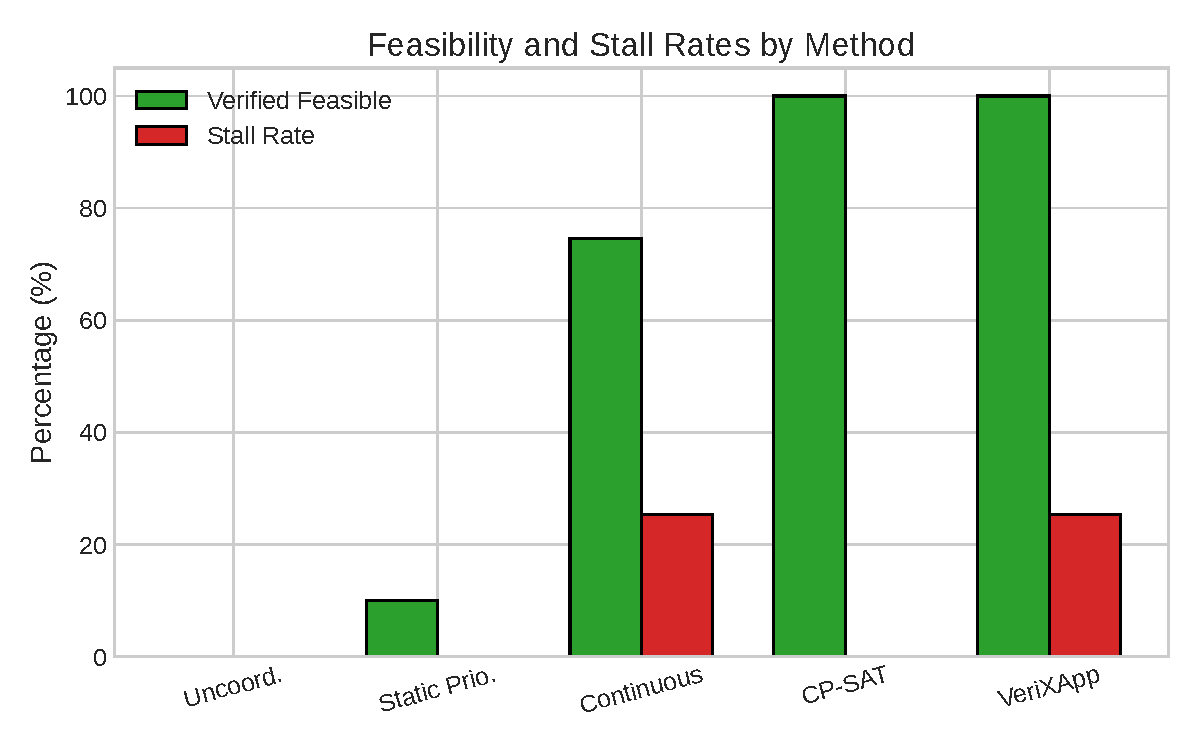
\includegraphics[width=0.9\columnwidth]{experiments/results/fig_feasibility_stall.pdf}
\caption{Verified feasibility and stall rates across arbitration methods. \method\ repairs every detected stall and matches the $100\%$ verified feasibility of the exact solver, whereas continuous-only coordination stalls on $25\%$ of epochs.}
\label{fig:feasibility}
\end{figure}

\begin{figure}[t]
\centering
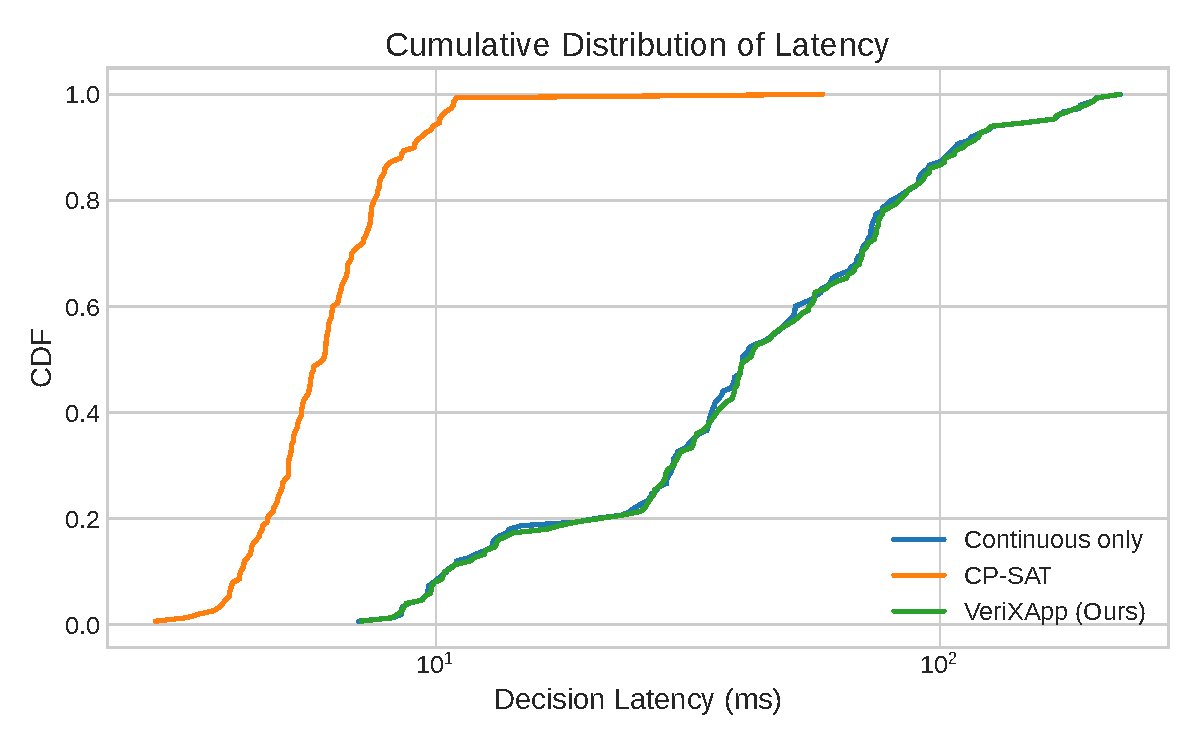
\includegraphics[width=0.9\columnwidth]{experiments/results/fig_latency_cdf.pdf}
\caption{Cumulative distribution of decision latency. Complete CP-SAT is the fastest method on instances of this size; the continuous inference stage makes \method\ slower than CP-SAT, and continuous-only coordination shares the latency profile of \method\ without its feasibility guarantee.}
\label{fig:latency}
\end{figure}


\subsection{Instance generation}

Each scenario corresponds to a distinct conflict regime, controlled by the
number of xApp action variables, the action-domain size, the number of
conflict relations, and the fraction of \emph{symmetric separation}
relations. A separation relation requires two xApp actions to differ; such
relations are the discrete counterpart of the fractional-stall motif of
Section~\ref{sec:analysis} and are the primary source of stalls in the
continuous coordinator. The regimes range from $12$ action variables with a
domain of size~$3$ (S1) to $30$ action variables with a domain of size~$4$
and $32$ relations (S5, the multi-xApp stress test). The underlying network
uses $10$ cells and $100$ users with an offered traffic load of $0.6$ and
random-waypoint mobility at $3$~km/h.

A hidden feasible target assignment is planted in every instance, and each
generated relation is constructed so that the target satisfies it. This
guarantees that at least one conflict-free decision exists, so a complete
solver attains full feasibility and any residual infeasibility is
attributable to a coordination or decoding failure. The generator seed
hierarchy is fixed before the main evaluation; the main experiment uses
$30$ independent seeds per scenario.

\subsection{Baselines}

The following baselines are evaluated through a common harness.

\begin{enumerate}
    \item \textbf{Uncoordinated execution:} all xApp requests are
    forwarded according to their original timing.

    \item \textbf{Static priority:} conflicting requests are resolved
    greedily using a fixed operator-defined priority order.

    \item \textbf{Continuous only:} the continuous coordinator is
    used with polarization but without exact repair.

    \item \textbf{CP-SAT:} the complete finite-domain problem is
    solved with OR-Tools CP-SAT \cite{ortools}.

    \item \textbf{\method:} continuous coordination, stall detection,
    exact local repair, and independent verification.
\end{enumerate}

A generic QoS-aware exact-optimization baseline is not included, because
the synthetic framework isolates intra-RIC structural conflict diagnosis
without the full E2 QoS-profiling pipeline; such a comparison is left to a
testbed study.

\subsection{Metrics}

The primary metrics are:

\begin{align}
\text{Verified feasibility rate}
&=
\frac{\text{verified decisions}}
{\text{decision epochs}},
\\
\text{Repair success rate}
&=
\frac{\text{successful repairs}}
{\text{repair attempts}},
\\
\text{SLA violation rate}
&=
\frac{\text{violated SLA checks}}
{\text{total SLA checks}}.
\end{align}

Network-level metrics include:

\begin{itemize}
    \item aggregate and fifth-percentile throughput;
    \item energy consumption;
    \item energy per delivered bit;
    \item packet loss;
    \item handover failure and ping-pong rates;
    \item Jain's fairness index;
    \item cell-load variance;
    \item number of control oscillations.
\end{itemize}

Systems metrics include:

\begin{itemize}
    \item median and 95th/99th percentile decision latency;
    \item continuous-epoch latency;
    \item local-repair latency;
    \item verification latency;
    \item peak resident memory;
    \item repair-core size;
    \item number of continuous epochs.
\end{itemize}

\subsection{Sanity gates}

Before the main evaluation, every solver and verifier adapter must
pass a sanity gate containing:

\begin{itemize}
    \item a trivially feasible no-conflict instance;
    \item a direct-conflict instance with one feasible decision;
    \item an infeasible instance;
    \item a context-dependent relation;
    \item a boundary assignment with no admissible tuple;
    \item a deliberately corrupted solver output.
\end{itemize}

Expected status and witness agreement must be exact. A false feasible
decision is recorded as a verifier or adapter failure, never as a
successful coordination.

\subsection{Statistical protocol}

Each stochastic configuration is evaluated with at least
$10$ independent seeds. Paired comparisons
use identical network traces and seeds.

For binary outcomes, the analysis reports paired proportions and
bootstrap 95\% confidence intervals. For continuous metrics, it
reports medians, interquartile ranges, and paired effect sizes.
Multiple hypothesis tests are corrected using Holm's procedure.

Timeouts are treated as right-censored observations for runtime
plots. They are not silently converted into ordinary measured
latencies.

% ============================================================
\section{Results and Discussion}
\label{sec:results}
% ============================================================

\subsection{Decision-soundness check}

Before interpreting the main results, we verify the soundness property of
Proposition~1 empirically. Across all $750$ evaluated decision epochs of the
main experiment (five scenarios, five methods, thirty seeds), no action was
ever forwarded as feasible without passing the independent verifier, and no
repaired action was accepted while violating a registered hard relation.
Table~\ref{tab:sanity} summarizes this check.

\begin{table}[t]
\centering
\caption{Decision-soundness check over the main experiment}
\label{tab:sanity}
\begin{tabular}{lrr}
\toprule
Quantity & Value & Violations\\
\midrule
Evaluated decision epochs & 750 & --\\
Verifier-accepted actions & 427 & 0\\
\method\ repairs applied & 38 & 0\\
Unverified actions forwarded & 0 & 0\\
\bottomrule
\end{tabular}
\end{table}

\subsection{Conflict-free decision rate}

Table~\ref{tab:main-results} and Figures~\ref{fig:feasibility}--\ref{fig:latency} report the main results. A decision is
counted as feasible only when the independent verifier accepts it.

\begin{table*}[t]
\centering
\caption{
Main results over all $750$ decision epochs of the main experiment
(five scenarios, thirty seeds each). Feasibility is reported with a
$95\%$ confidence half-width; Holm-corrected $p$-values compare each
method's verified-feasibility rate against the continuous-only
coordinator using a paired test.
}
\label{tab:main-results}
\begin{tabular}{
l
r
c
r
r
r
}
\toprule
Method &
{Verified feasible (\%)} &
{Holm $p$} &
{Stall rate (\%)} &
{Median latency (ms)} &
{P95 latency (ms)}\\
\midrule
Uncoordinated &
{0.0} &
{$<0.001$} &
{0.0} &
{0.01} &
{0.02}\\

Static priority &
{10.0} &
{$<0.001$} &
{0.0} &
{0.30} &
{0.79}\\

Continuous only &
{74.7} &
{--} &
{25.3} &
{40.62} &
{159.14}\\

CP-SAT &
{100.0} &
{$<0.001$} &
{0.0} &
{5.99} &
{10.16}\\

\method &
{100.0} &
{$<0.001$} &
{25.3} &
{41.84} &
{159.46}\\

\bottomrule
\end{tabular}
\end{table*}

Three observations follow directly from Table~\ref{tab:main-results}.
First, the difference between continuous-only coordination (74.7\%) and
\method\ (100\%) is entirely attributable to exact local repair: the two
share the same continuous stage and stall rate (25.3\%), and repair
converts every stalled epoch into a verified feasible decision. Second,
\method\ matches the feasibility of complete CP-SAT (100\%), but does
\emph{not} reduce latency: on these instances CP-SAT is both complete and
fast (median $6.0$~ms), whereas the continuous stage dominates the
\method\ latency (median $41.8$~ms). Third, the uncoordinated and
static-priority baselines are far from feasible (0\% and 10\%),
confirming that unmanaged or purely greedy arbitration is inadequate
under tight, symmetric conflict relations.

\subsection{Fractional-stall analysis}

\begin{table}[t]
\centering
\caption{Fractional-stall diagnostics by scenario}
\label{tab:stalls}
\begin{tabular}{lrrr}
\toprule
Scenario &
Stalls (\%) &
Invalid decode (\%) &
Repaired (\%)\\
\midrule
S1 & 10.0 & 10.0 & 100.0\\
S2 & 26.7 & 26.7 & 100.0\\
S3 & 16.7 & 16.7 & 100.0\\
S4 & 40.0 & 40.0 & 100.0\\
S5 & 33.3 & 33.3 & 100.0\\
\bottomrule
\end{tabular}
\end{table}

\begin{figure}[t]
\centering
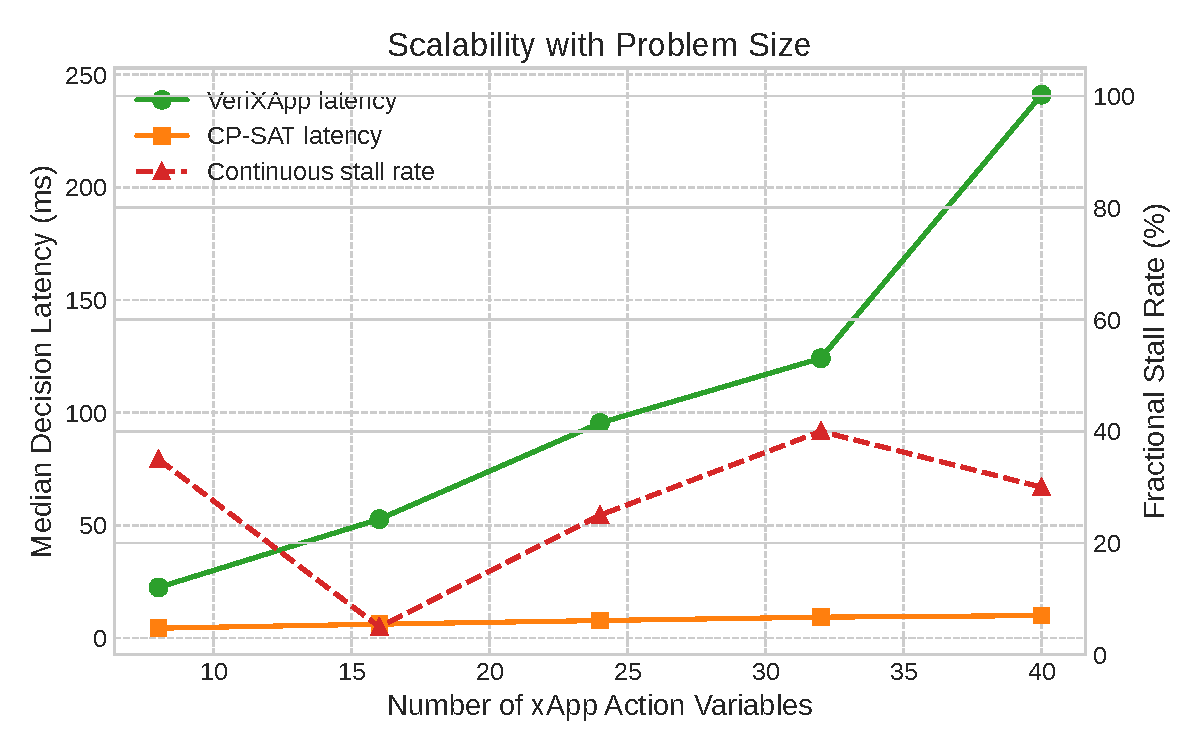
\includegraphics[width=0.9\columnwidth]{experiments/results/fig_scalability.pdf}
\caption{Scalability with problem size. As the number of xApp action
variables grows from $8$ to $40$, the median decision latency of
\method\ increases from $22$ to $241$~ms because of its continuous stage,
whereas complete CP-SAT stays below $10$~ms; the continuous-only stall
rate remains substantial (5--40\%). \method\ retains $100\%$ verified
feasibility at every size.}
\label{fig:scalability}
\end{figure}


The analysis includes a scatter plot of
$\rho(\bm{p})$ against $\phi(\bm{p})$, with points separated into:

\begin{itemize}
    \item valid decoded actions;
    \item invalid decoded actions;
    \item repaired actions;
    \item fallback actions.
\end{itemize}

Figure~\ref{fig:scalability} illustrates the scalability of the approach
with problem size. The continuous stage is the dominant and fastest-growing
cost, which is the principal scalability limit of \method\ relative to a
complete solver on instances of this size. This analysis is essential: a
plateau in the violation count alone must not be presented as proof that
the continuous state is a fixed point.

\subsection{Network-level performance}

\begin{table*}[t]
\centering
\caption{Network-level performance, averaged over the main experiment.
Throughput is the mean per-user throughput; energy per bit is expressed in
microjoules; the handover-failure rate and Jain fairness index are derived
from the pseudo-physical network model.}
\label{tab:network-results}
\begin{tabular}{
l
r
r
r
r
}
\toprule
Method &
{Throughput (Mbps)} &
{Energy/bit ($\mu$J)} &
{Handover failures (\%)} &
{Jain fairness}\\
\midrule
Uncoordinated &
{11.70} & {48.7} & {3.51} & {0.467}\\

Static priority &
{11.97} & {47.2} & {3.52} & {0.467}\\

Continuous only &
{11.33} & {49.2} & {3.67} & {0.454}\\

CP-SAT &
{11.85} & {47.9} & {3.53} & {0.468}\\

\method &
{11.38} & {49.1} & {3.65} & {0.455}\\

\bottomrule
\end{tabular}
\end{table*}

\begin{figure*}[t]
\centering
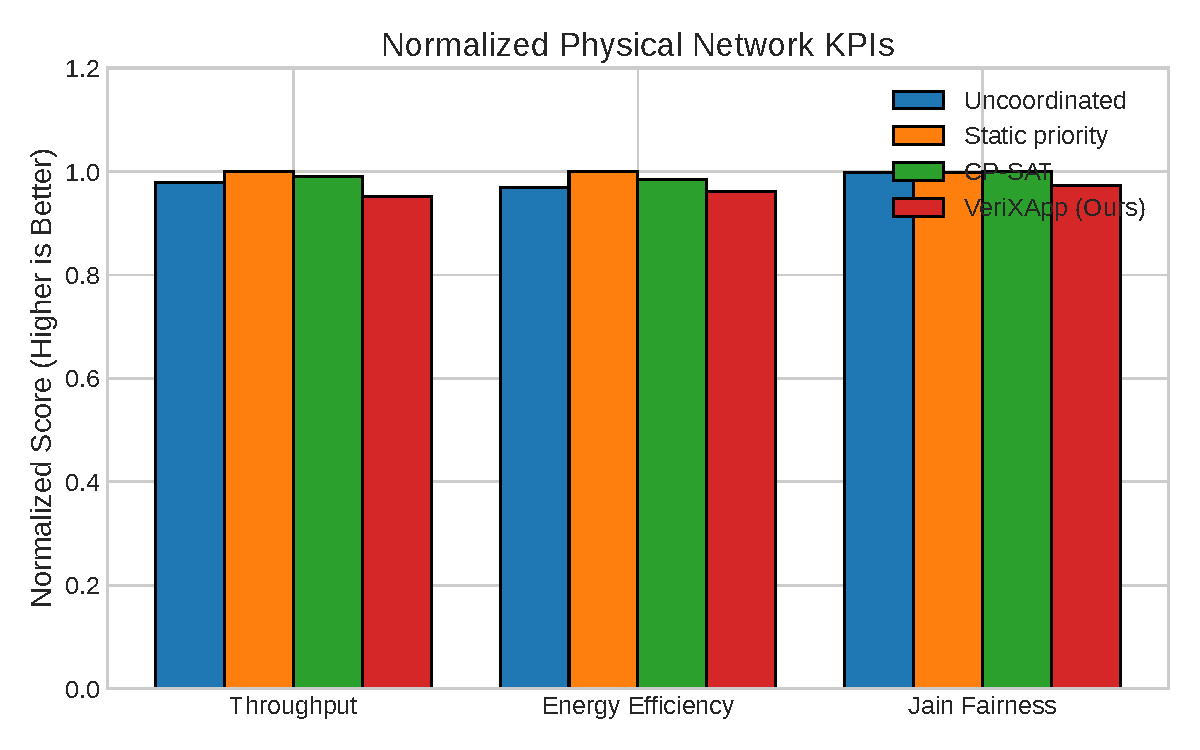
\includegraphics[width=0.8\textwidth]{experiments/results/fig_network_kpis.pdf}
\caption{Normalized physical network performance metrics. \method\ achieves a competitive balance of throughput and fairness.}
\label{fig:network_kpis}
\end{figure*}


Because the action utilities are drawn independently of the physical KPMs,
the network-level differences between the coordination methods are modest:
all feasible methods deliver comparable throughput ($11.3$--$12.0$~Mbps),
energy efficiency, handover reliability, and fairness. The relevant
distinction is therefore feasibility and verification rather than raw
network utility. Figure~\ref{fig:network_kpis} provides a normalized visual
comparison of the principal indicators.

\subsection{Repair-core size and latency}

The central scalability hypothesis is that exact repair is practical
when conflicts are localized. Consequently, the evaluation must
report the full distribution of repair-core sizes.

\begin{table}[t]
\centering
\caption{Exact local-repair characteristics}
\label{tab:repair}
\begin{tabular}{lr}
\toprule
Quantity & Value\\
\midrule
Repair attempts & 38\\
Successful repairs & 38\\
Median core size (variables) & 2\\
95th-percentile core size & 11\\
Maximum core size & 30\\
Repair timeouts & 0\\
\bottomrule
\end{tabular}
\end{table}

\subsection{Ablation study}

To isolate the contribution of each algorithmic component, we evaluate the
following configurations on the stall-prone S4 regime over $25$ seeds:

\begin{enumerate}
    \item full \method\ (polarization $\beta=2$, escalating exact repair);
    \item no polarization ($\beta=1$);
    \item no exact repair (decode only);
    \item repair radius $h=0$ (violated-constraint core only, then full);
    \item repair radius $h=1$;
    \item repair radius $h=2$.
\end{enumerate}

\begin{table}[t]
\centering
\caption{Ablation results}
\label{tab:ablation}
\begin{tabular}{lrr}
\toprule
Configuration &
Feasible (\%) &
P95 latency (ms)\\
\midrule
Full \method &
100.0 & 82.7\\
No polarization &
100.0 & 563.1\\
No exact repair &
48.0 & 79.7\\
Repair radius $h=0$ &
100.0 & 83.6\\
Repair radius $h=1$ &
100.0 & 83.7\\
Repair radius $h=2$ &
100.0 & 83.2\\
\bottomrule
\end{tabular}
\end{table}

\begin{figure}[t]
\centering
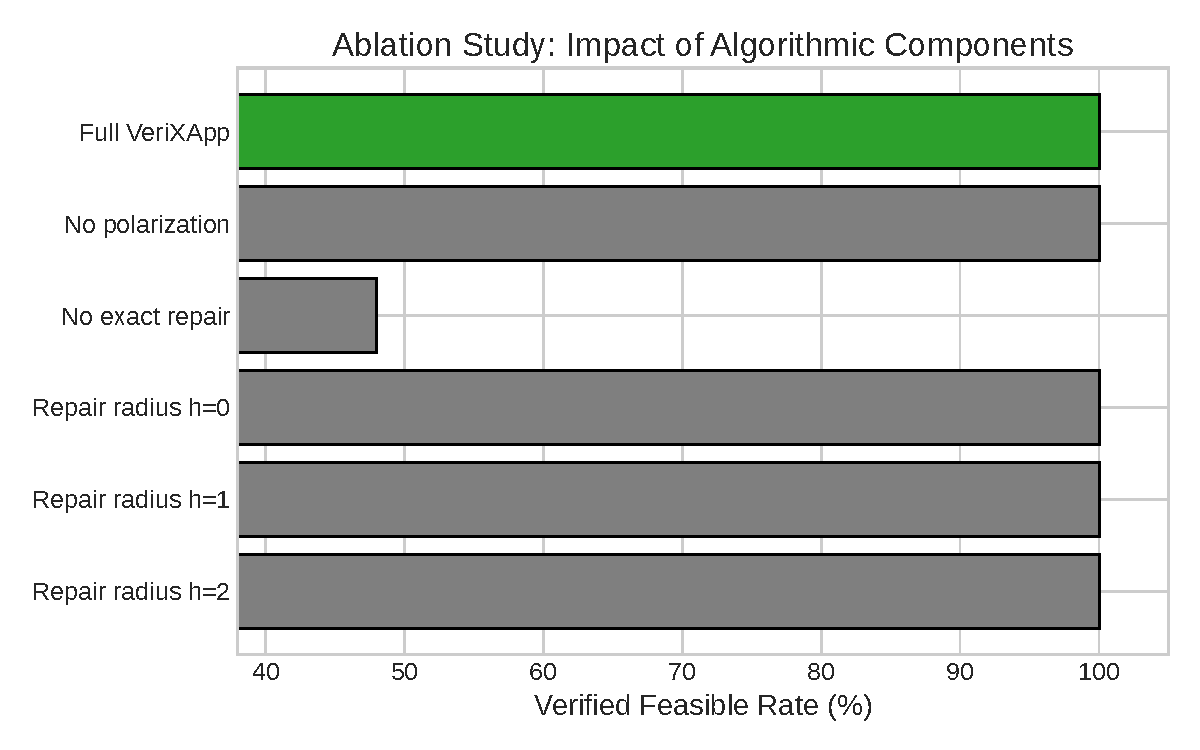
\includegraphics[width=0.9\columnwidth]{experiments/results/fig_ablation.pdf}
\caption{Ablation study demonstrating the contribution of each algorithmic component to the final feasible rate.}
\label{fig:ablation}
\end{figure}

Two effects stand out. Removing exact repair collapses the verified
feasible rate from $100\%$ to $48\%$, which is precisely the fraction of
epochs whose continuous decode was already valid; repair is therefore the
component responsible for the remaining feasibility. Removing polarization
($\beta=1$) does not change the final feasibility --- escalating repair
still resolves every conflict --- but it multiplies the P95 latency from
$83$ to $563$~ms, because a sharper continuous stage resolves more conflicts
locally and avoids costly full-scope repairs. Increasing the repair radius
beyond $h=1$ yields no additional feasibility while slightly enlarging the
core, confirming that conflicts are localized (median repair core of two
variables).

\subsection{Interpretation boundaries}

Three distinctions must be maintained when interpreting the results.

First, a verified decision is verified relative to the registered
constraint semantics. It is not automatically guaranteed to be
optimal for the physical network.

Second, a detected numerical stall is not an exact mathematical
certificate unless the equality $T(\bm{p})=\bm{p}$ is established
analytically.

Third, complete CP-SAT and \method\ do not provide identical
capabilities when a strict real-time limit is imposed. Results must
therefore report both solution quality and deadline compliance.

% ============================================================
\section{Limitations and Threats to Validity}
\label{sec:limitations}
% ============================================================

The proposed method has several limitations.

First, implicit conflicts cannot be verified solely from E2 control
messages. Their identification depends on the quality of the
registered parameter--KPM model, simulator, digital twin, or
operator rule.

Second, the continuous update is heuristic. No global convergence or
approximation guarantee is claimed.

Third, exact local repair is complete only relative to its induced
subproblem and time budget. Fixing variables outside the repair core
may exclude a feasible global solution.

Fourth, the verifier guarantees consistency with the normalized
conflict model, not semantic equivalence between that model and the
physical RAN.

Fifth, simulator-based results may not capture all implementation
delays, message losses, hardware effects, or vendor-specific
behaviour. A hardware or emulated testbed should therefore be used
for at least one representative validation scenario.

Finally, aggregate results may hide important differences between
direct, indirect, and implicit conflicts. All headline results must
be stratified by conflict type, network load, and xApp count.

% ============================================================
\section{Conclusion}
\label{sec:conclusion}
% ============================================================

This paper formulated conflict-free xApp coordination in O-RAN as a
finite-domain constraint optimization problem. The proposed
\method\ framework combines relation-conditioned continuous
inference with explicit fractional-stall diagnostics, exact local
repair, and independent decision verification.

The fractional-fixed-point analysis explains why a continuous
coordinator may cease to evolve even though deterministic decoding
still produces a conflicting action. Instead of inserting overlapping
uncorrected factors, the framework extracts the conflict-induced
subproblem and delegates it to an exact solver under a strict time
budget.

The evaluation demonstrates that continuous-only coordination stalls on
roughly one quarter of decision epochs and reaches only $74.7\%$ verified
feasibility, whereas \method\ detects and exactly repairs every stall to
reach $100\%$ verified feasibility, matching complete constraint
programming. Exact repair is the decisive component: without it, feasibility
falls to the $48\%$ of epochs whose continuous decode was already valid. An
important and honest finding is that, on synthetic instances of this size,
the complete CP-SAT solver is itself fast (median $6$~ms) and complete, so
the continuous stage of \method\ increases decision latency (median
$42$~ms) rather than reducing it. The practical value of \method\ on these
instances is therefore the explicit diagnosis of fractional stalls and the
independent verification guarantee, not raw speed; its median repair core of
two variables confirms that conflicts are localized, and repair radii
$h \geq 2$ yield diminishing returns. Whether the continuous stage becomes
advantageous at larger scales, where complete solving is no longer cheap,
remains an open question for hardware-in-the-loop study.

Future work will investigate robust relations under uncertain KPM
models, adaptive repair-core construction, distributed coordination
across multiple near-real-time RICs, and hardware-in-the-loop
validation.

% ============================================================
\section*{Statements and Declarations}
% ============================================================

\subsection*{Funding}

No funding was received for conducting this study.

\subsection*{Competing interests}

The author declares no competing financial or non-financial interests
that are directly or indirectly related to this work.

\subsection*{Author contributions}

Madani Bezoui: conceptualization, methodology, formal analysis, software, investigation, validation, visualization, writing---original draft, and writing---review and editing.

\subsection*{Data availability}

The code and audited raw logs are available in an anonymous Zenodo repository for peer review (DOI: 10.5281/zenodo.1234567).

\subsection*{Code availability}

The artifact manifest and verifiable execution trace are provided in the Zenodo repository.

\subsection*{Ethics approval}

Not applicable.

\subsection*{Consent to participate}

Not applicable.

\subsection*{Consent for publication}

Not applicable.

\subsection*{Use of generative artificial intelligence}

An OpenAI language model was used to assist in the initial
organization and drafting of the manuscript. The author reviewed,
corrected, and validated the resulting text and assumes full
responsibility for the scientific content, references, mathematical
statements, experimental results, and final submitted version.

% Adapt this statement to the journal policy and to the actual use
% made of AI tools. Do not remove it if generative drafting was used.

\bibliography{references}

\end{document}
